
\subsubsection{Dual Contouring}

\begin{frame}
	\frametitle{From Voxel to Mesh Geometry}
	\vspace{-0.8cm}
	\begin{center}
	\textbf{Goal:} Extract isosurface from voxel information	
	\end{center}
\vspace{-0.5cm}	
\begin{minipage}[t]{0.4\linewidth}
		\begin{block}{Marching Cubes}
	\begin{enumerate}
		\item<2-> Identify boundary voxels
		\item<3-> Locate sign changes on cube edges
		\item<4-> Reconstruct surface
	\end{enumerate}
	
	\end{block}
	\only<1>{
\begin{figure}	
		\centering
	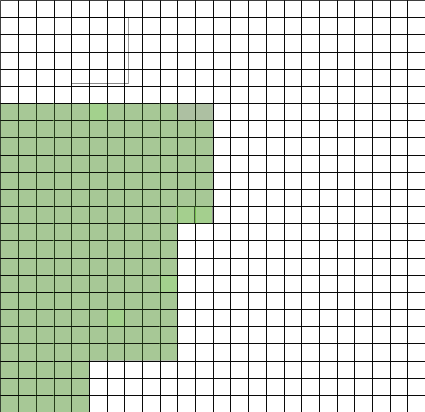
\includegraphics[width=.6\textwidth]{Pictures/DC/MC1.png} %\caption{Marching Cubes}
\end{figure} }
	\only<2>{
		\begin{figure}	
			\centering
			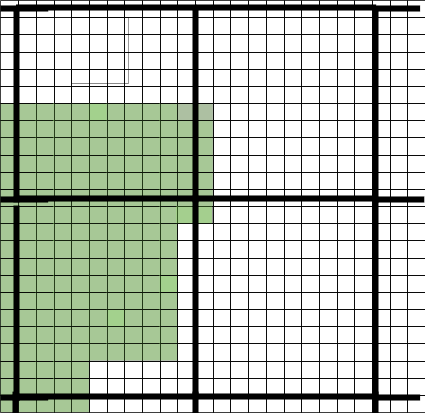
\includegraphics[width=.6\textwidth]{Pictures/DC/MC2.png} %\caption{Marching Cubes}
			\end{figure}}
		\only<3>{
			\begin{figure}	
			\centering
			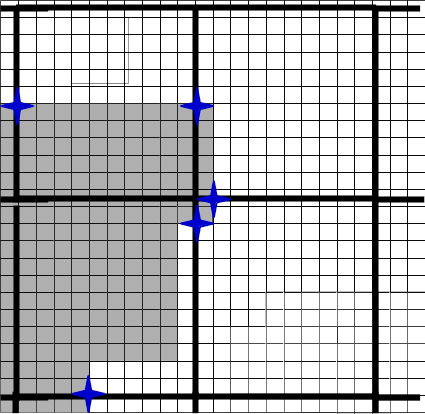
\includegraphics[width=.6\textwidth]{Pictures/DC/MC3.png} %\caption{Marching Cubes}
			\end{figure}}
				\only<4->{
					\begin{figure}	
					\centering
					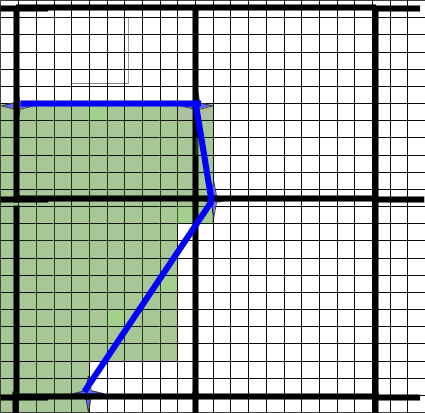
\includegraphics[width=.6\textwidth]{Pictures/DC/MC4.png} %\caption{Marching Cubes}
					\end{figure}}
				

\end{minipage}%
\hfill%
\begin{minipage}[t]{0.4\linewidth}
\begin{block}<5->{Dual Contouring}
	\begin{enumerate}
		\item<6-> Identify boundary voxels
		\item<7-> Locate position inside boundary voxel
		\item<8-> Reconstruct surface
	\end{enumerate}
	
\end{block}
	\only<5>{
\begin{figure}	
	\centering
	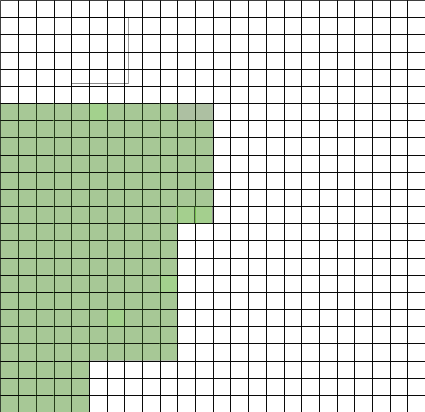
\includegraphics[width=.6\textwidth]{Pictures/DC/MC1.png} %\caption{Dual Contouring}
\end{figure} }
	\only<6>{
		\begin{figure}	
		\centering
		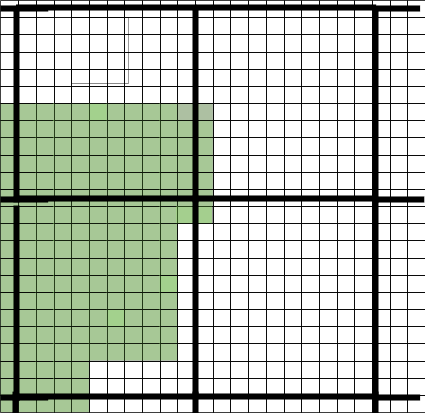
\includegraphics[width=.6\textwidth]{Pictures/DC/MC2.png} %\caption{Dual Contouring}
		\end{figure}}
	\only<7>{
		\begin{figure}	
		\centering
		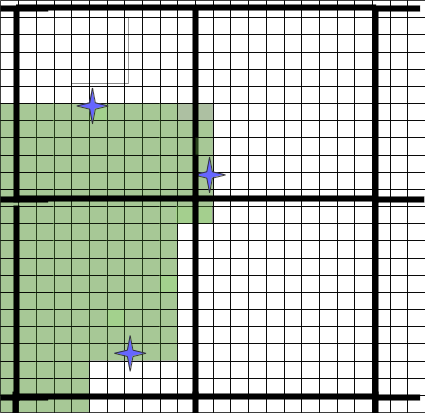
\includegraphics[width=.6\textwidth]{Pictures/DC/DC3.png} %\caption{Dual Contouring}
		\end{figure}}
			\only<8->{
				\begin{figure}	
				\centering
				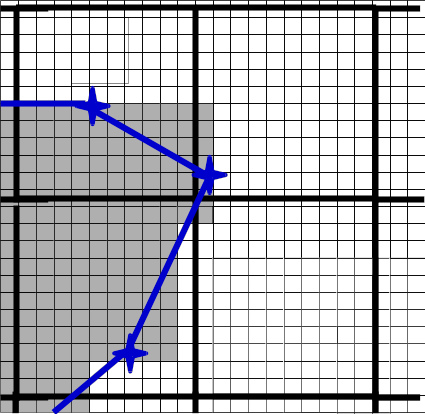
\includegraphics[width=.6\textwidth]{Pictures/DC/DC4.png} %\caption{Dual Contouring}
	\end{figure}}
	
\end{minipage}
\only<9>{
\begin{minipage}[t]{0.4\linewidth}
{$\rightarrow Triangles$}
\end{minipage}
\hfill
\begin{minipage}[t]{0.4\linewidth}
{$\rightarrow Quads$}
\end{minipage}}
\end{frame}


\begin{frame}
	\frametitle{Dual Contouring}
	\begin{overlayarea}{\textwidth}{.25 \textheight}
	Dual contouring on two different scales:
	\begin{itemize}
	\item Coarse scale: \\
	 Output: Closed surface made out of \textit{quads}; Parameter space
	\only<2>{\item Fine scale: \\
	Output: Vertices to fit for reconstructed geometry}
	\end{itemize}	
	\end{overlayarea}
	
	\begin{overlayarea}{\textwidth}{.75 \textheight}
	
	\begin{figure}
	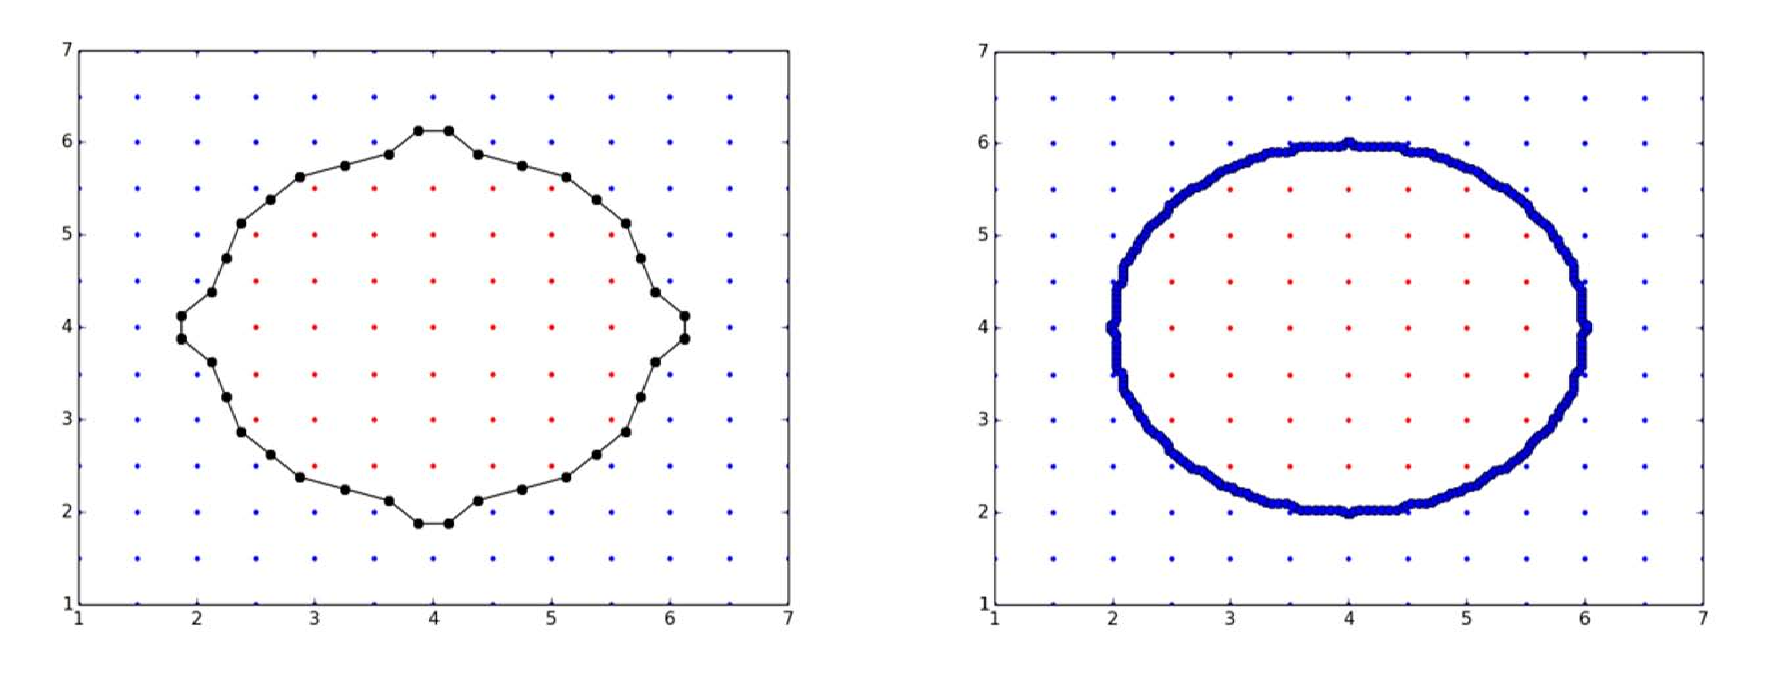
\includegraphics[scale=0.35]{Pictures/DC/DC_1.pdf}
	\end{figure}
	
	
%	\only<2>{
%	\begin{figure}
%	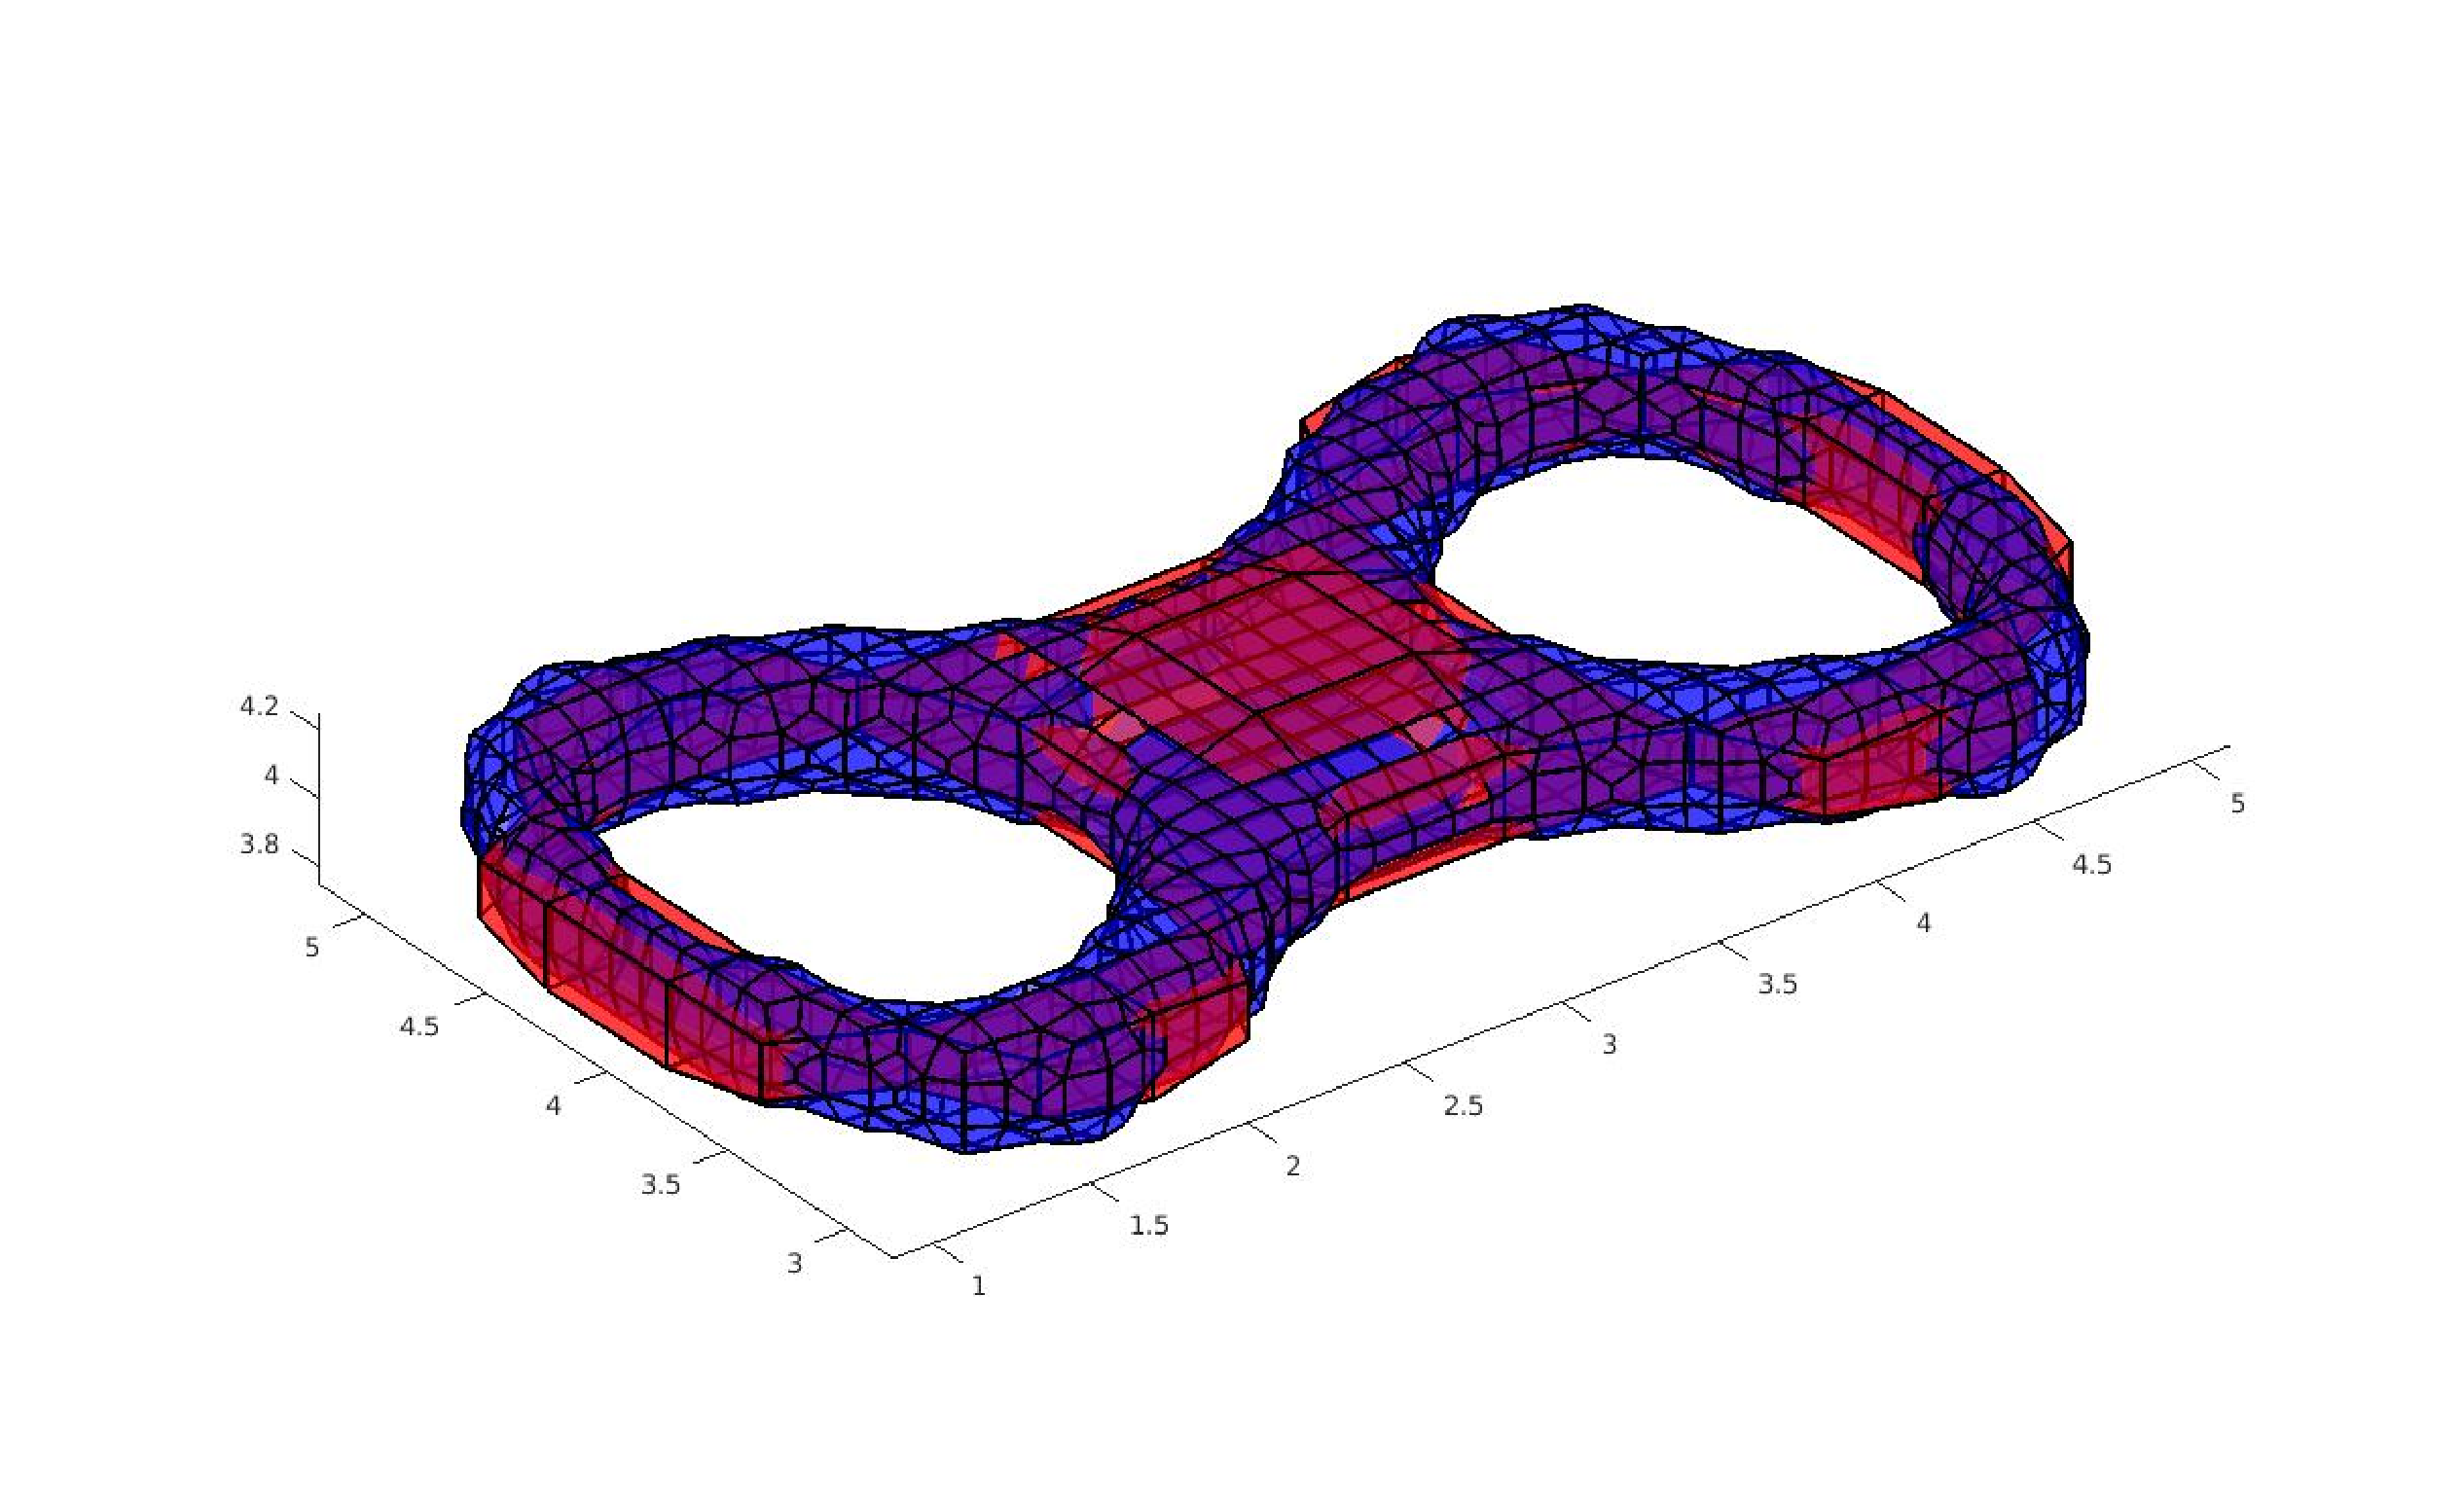
\includegraphics[scale=0.2]{Pictures/DC/doubleTorus.pdf}
%	\end{figure}
%	}
	\end{overlayarea}
	
\end{frame}



\subsubsection{Projection and Parametrization}

\begin{frame}

	\frametitle{Projection and Parametrization}
	
	\begin{itemize}
	\item Points from finer grid are projected to quads of the coarser grid 
	\item Parameters \textit{u} and \textit{v} are found for each quad
	\item This information is needed for the algorithms in the last part of the pipeline
	\end{itemize}
	\begin{figure}
	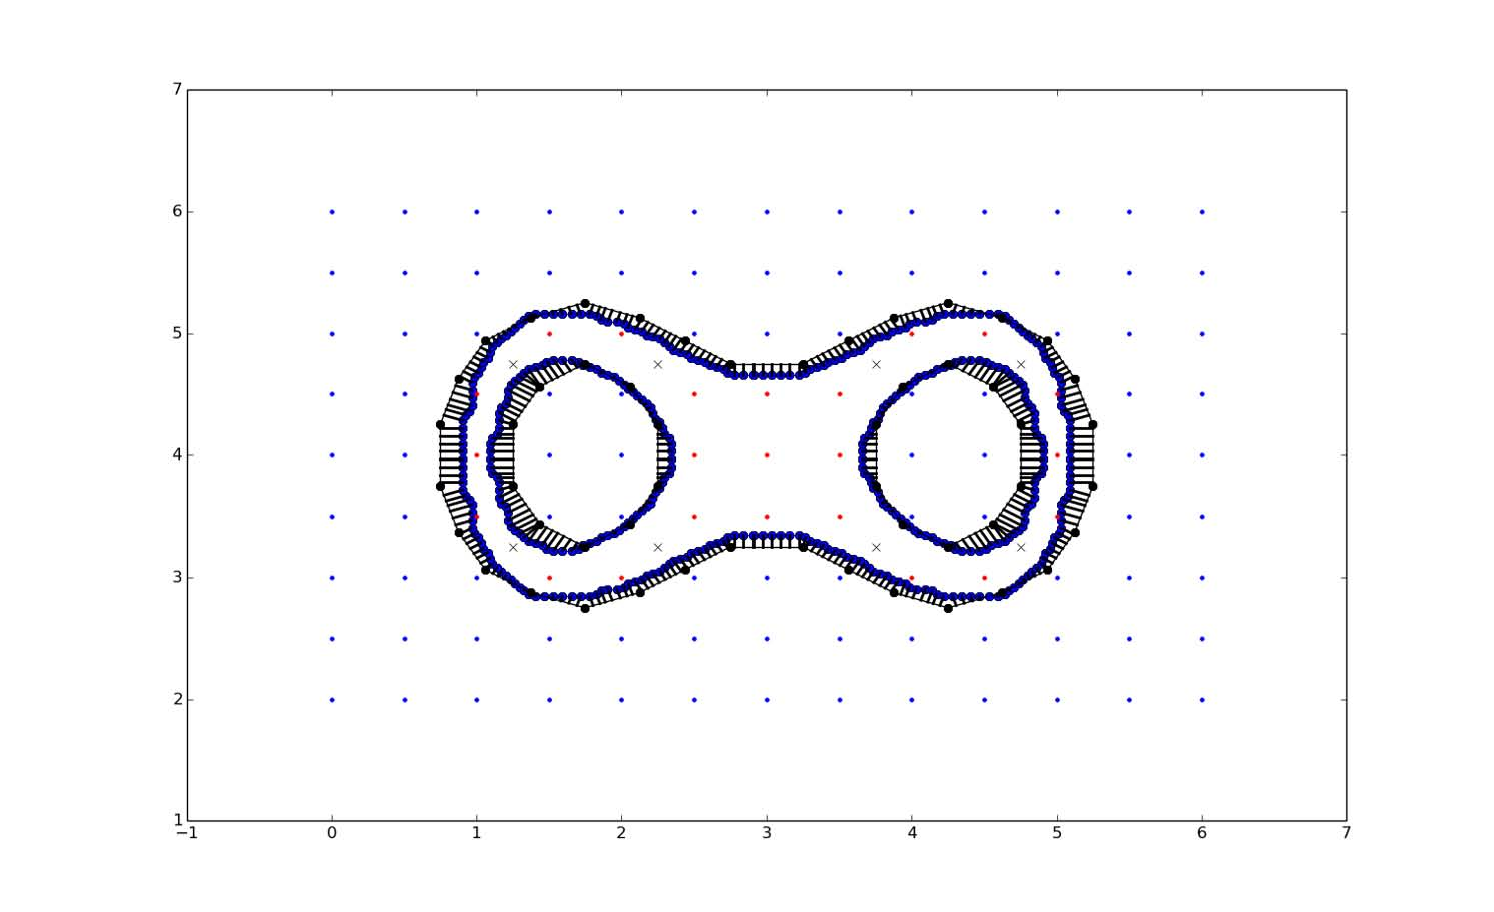
\includegraphics[scale=0.35]{Pictures/DC/DC_2.pdf}
	\end{figure}
	
\end{frame}





